Sensitivity studies presented in Section~\ref{sec:physics-lbnosc-senscalc} test the ability to distinguish
the expected number of \nue appearance and \numu disappearance events, given a set of oscillation parameters,
from the expectations given an alternate set of parameters. For example, the CP violation and MH sensitivity
studies test the spectral differences induced by shifting \deltacp away from 0.0 and $\pi$ and by changing the
mass hierarchy, quantifying these differences with a test statistic. This test statistic includes the effect of
both statistical differences and
systematic uncertainties. The effect of systematic uncertainty in the parameters governing these spectra
is included by allowing the paramaters to vary within gaussian ranges and profiling over 
these systematic nuisance parameters in the fit, i.e. the set of nuisance parameters that produces the
lowest total value of the test statistic is chosen.  The central values and 1$\sigma$ uncertainties on the oscillation
parameters are taken from the Nu-Fit~\cite{Gonzalez-Garcia:2014bfa} global fit to neutrino data; the values are
given in Table~\ref{tab:oscpar_nufit}. Uncertainty in the non-oscillation parameters is approximated using
normalization uncertainties on each constituent interaction mode that comprise the signal and background
interactions in each sample. These normalization uncertainties are chosen based on
current constraints on underlying model parameters, the ability of previous experiments to constrain
these quantities, and the expected ability of the DUNE Near Detector (ND) as outlined in Section~\ref{reftoND}.
Consideration is also given to the sources of uncertainty that go into each of the effective normalization
parameters and how they may be correlated among the Far Detector (FD) analysis samples that will be fit in
combination.

In the sensitivities presented in Section ~\ref{sec:physics-lbnosc-senscalc},
the \nue and \anue signal normalization uncertainties are $5\% \oplus 2\%$, implemented as
5\% signal normalization uncertainties on the \numu and \anumu samples and
2\% on the \nue and \anue samples. These four signal normalization uncertainties
are treated as 100\% uncorrelated so that the 2\% normalization uncertainty on the
\nue sample represents a residual normalization uncertainty after constraints
from the near detector, the \numu disappearance samples, and the \anue sample have been applied.
The normalization uncertainties on background to these samples and the correlation among those
uncertainties are presented in Table~\ref{tab:bgnormsys}. The result of the correlations
described in Table~\ref{tab:bgnormsys} is that there are five independent background
normalization uncertainties: beam \nue, beam \anue, \numu/NC background to appearance mode,
NC background to disappearance mode, and $\nu_\tau$. 

\begin{table}[!tb]
  \begin{center}
    \caption{Normalization uncertainties and correlations for background to the \nue, \anue, \numu, and \anumu data samples.}
    \label{tab:bgnormsys}
    \begin{tabular}{l|c|l} \hline\hline
      Background & Normalization Uncertainty & Correlations \\ \hline
      \multicolumn{3}{l}{For \nue/\anue appearance:} \\ 
      Beam \nue & 5\% & Uncorrelated in \nue and \anue samples \\
      NC      & 5\%  & Correlated in \nue and \anue samples \\
      \numu CC & 5\% & Correlated to NC \\
      $\nu_\tau$ CC & 20\% & Correlated in \nue and \anue samples \\ \hline
      \multicolumn{3}{l}{For \numu/\anumu disappearance:} \\ 
      NC & 5\% & Uncorrelated to \nue/\anue NC background \\
      $\nu_\tau$ & 20\% & Correlated to \nue/\anue $\nu_\tau$ background \\
    \end{tabular}
  \end{center}
  \end{table}

In the following sections, we present a justification for the chosen values of the signal and background
normalization uncertainties and we consider the effect of varying the size of the residual normalization
uncertainties on the \nue and \anue samples.We also describe the ongoing effort to characterize and evaluate the effect of individual sources
of uncertainty in the DUNE experiment.

\subsection{Justification of Normalization Uncertainties}
\label{sec:syst_just}
Uncertainties in DUNE will be constrained by external data, near detector data, and the combined
fit to the four (\nue, \anue, \numu, \anumu) far detector samples.
The \numu disappearance analysis sample is composed of \numu CC interactions with background from NC
interactions in which a charged pion is misidentified a muon and $\nu_{\tau}$ CC interactions in which the resulting
tau decays to a muon and two neutrinos.
The unoscillated \numu flux is expected to be well-constrained by the near detector.
The uncertainty on the neutral current background comes primarily from uncertainty in pion production rates
for the coherent, resonance and DIS channels.
%The charged pion misidentification rate, and its associated
%uncertainty, is highly correlated with the fraction
%of pions that either exit the detector, are absorbed by nuclei, or expend their kinetic before interacting
%hadronically, and thus have the topological characteristics of a muon.
%These relative rates of these processes will be constrained by the ND.
Uncertainties in the $\nu_{\tau}$ CC background level arise from the uncertainty in the $\nu_{\tau}$/\numu
cross-section ratio, which cannot be constrained by ND measurements.

The \nue appearance sample is composed of electron neutrinos resulting from \numu$\rightarrow$\nue oscillation,
intrinsic beam \nue, NC or \numu CC interactions in which a photon from a final-state neutral pion is
misidentified as an electron, and $\nu_{\tau}$ interactions in which the tau decays to an electron and
two neutrinos. Since the
\numu disappearance signal and the \nue appearance signal are produced by the same flux, flux uncertainty is
constrained in the three-flavor fit;
%For example, changing the flux will increase the relative rates of the numu and nue samples the amount,
%while adjusting q23 will cause one sample to rise and the other to fall.
the correlated uncertainties between the \nue and \numu samples will cancel, leaving only residual uncorrelated
uncertainties which result from differences in energy scale and selection efficiency between the samples,
as well as theoretical uncertainties on the \nue/\numu cross-section ratio. The uncertainty on the intrinsic
beam \nue background is dominated by flux uncertainties which are constrained by the near detector.
Predictions for neutral current and \numu CC background rates are again limited by the uncertainties on pion
production rates.
%There are correlations between the charged and neutral pion production rates, allowing for
%cancellation of uncertainty in this background between the \nue and \numu samples.
%However, to be conservative the NC+CCnumu backgrounds in the nue are allowed to vary by an additional
%uncorrelated 5% to account for differences in pi0/pi+- production rates, and detection/selection efficiencies.
The $\nu_{\tau}$ background uncertainties are again related to cross-section ratio uncertainties
which are 100\% correlated among samples.

Energy scale uncertainties, which can affect the shape of the reconstructed energy spectra, result from
inaccurate models of detector response, missing energy in the hadronic systems (primarily from neutron production),
and from FSI. Since the dominant source of uncertainty is the hadronic energy scale which is the same for both
signal samples, the relative energy scale uncertainties are limited to differences in kinematics
between \numu and \nue interactions and differences in detector response for muons and electrons,
which will be highly constrained by test beam experiments.

Additional constraints are expected to occur in a fit to both neutrino and antineutrino beam samples;
variations in \deltacp induce opposite effects (in both shape and rate) in the \nue and \anue samples,
while most systematic uncertainties have a positively correlated effect.
The only systematic uncertainty thought to be able to induce an anti-correlated response between the \nue and \anue
samples comes from FSIs. This will require careful constraint from ND analysis, external data, and comparisons of
\nue to \numu and \anue to \anumu samples, where the peak of the appearance and the trough of the
disappearance samples must be the same. 
%% Similar arguments can be made for the antineutrino (RHC) beam samples, and therefore the same effective normalization uncertainties are used. The choice of uncertainties on the effective normalization parameters also reflect the significant cancellations achieved in the 4-sample fit resulting from the addition of 1) relating the nuebar app samples to the numubar dis samples, and 2) from the fact that variations in dcp induce opposite effects (in both shape and rate) in nue and nuebar samples, while most systematics have a positively correlated effect. In these choices it is conservatively assumed that the nu (FHC) flux and the nubar (RHC) flux are not correlated. The only systematic thought to be able to induce an anti-symmetric response between the nue and nuebar samples comes from FSIs. This will require careful constraint from ND analysis, external data, and comparisons of nue to numu, and nuebar to numubar, where the peak of the appearance and the trough of the disappearance samples must be the same. 


Based on these considerations and experience from previous and currently-running neutrino oscillation 
experiments, we believe that $5\% \oplus 2\%$ signal normalization (where 5\% is the normalization uncertainty on the
FD \numu sample and 2\% is the effective uncorrelated uncertainty on the FD \nue sample after fits to both near
and FD detector data and all external constraints) and normalization uncertainties on background as given
in Table \ref{tab:bgnormsys} are reasonably achievable in DUNE given a capable near detector with argon targets.
Table~\ref{tab:nuesysts} shows the uncertainties in a \nue appearance analysis achieved by MINOS~\cite{Adamson:2013ue} 
and T2K~\cite{Abe:2015awa} and compares the expected uncertainty in
DUNE. The goal uncertainties in DUNE are chosen by determining which
of the existing experiments is more representative of DUNE for each source
of systematic uncertainty and then setting a reasonable goal for a next-generation
experiment. These goals are based on the expected capabilities of the high-resolution
LAr TPC and  precise measurements from a highly-capable near detector, as well as
understanding of the analysis techniques employed by previous experiments.
A brief explanation of each choice in Table~\ref{tab:nuesysts} follows.
%
\begin{table}[!hb]
\begin{center}
  \caption {The dominant systematic uncertainties on the $\nu_e$-appearance 
    signal prediction in MINOS and T2K and a conservative projection of the 
    expected uncertainties in DUNE. In each case, the quoted uncertainty is
    the effect on the $\nu_e$-appearance signal only. These uncertainties 
    are the \emph{total} expected uncertainties on the $\nu_e$-appearance signal 
    which include both correlated and uncorrelated uncertainties in the 
    three-flavor fit. For reference, the uncertainties assumed in the nominal
    DUNE sensitivity calculations are also provided.\vspace{2pt}}
\label{tab:nuesysts}
\begin{tabular}{|l|c|c|c|l|} \hline\hline
Source of & MINOS & T2K & DUNE & Comments \\ \hline\hline
\multicolumn{5}{|c|}{Flux}  \\ \hline
Uncertainty & $\nu_e$ & $\nu_e$ & $\nu_e$ & \\ \hline\hline
Beam Flux & 0.3\% & 3.2\% & 2\% & See ``Flux Uncertainties'' in Section \ref{sec:syst_just_flux}\\
after N/F & & & & \\
extrapolation & & & & \\ \hline\hline
\multicolumn{5}{|c|}{Neutrino interaction modeling}  \\ \hline
Simulation & 2.7\% & 4.7\% & $\sim 2\%$ & See ``Simulation Uncertainties'' in Section \ref{sec:syst_just_sim} \\
includes: & & & & \\
hadronization & & & &  \\ 
cross sections & & & & \\ 
nuclear models & & & & \\ 
& & & & \\ \hline\hline
\multicolumn{5}{|c|}{Detector effects}  \\ \hline
Energy scale  & 3.5\% & included& (2\%) & Included in 5\% $\nu_\mu$ sample\\ 
($\nu_\mu$) & & above & &  normalization uncertainty in DUNE 3-flavor fit. \\ \hline
Energy  scale & 2.7\% & 2.5\% & 2\% & See ``\nue Energy Scale Uncertainties''\\
($\nu_e$) & & includes & &  in Section\ref{sec:syst_just_fd}\\
 & & all FD & & \\
 & & effects & & \\ \hline 
Fiducial & 2.4\% & 1\% & 1\% & Larger detectors = smaller uncertainty. \\ 
volume & & & & \\ \hline\hline
Total  & 5.7\% & 6.8\% & 3.6 \% & Residual $\nu_e$ uncertainty in  \\ 
& & & & full DUNE 3-flavor fit = 1-2\%. \\ \hline\hline
Used in DUNE & & & $5\% \oplus 2\%$ & 2\% \\
Sensitivity & & & & \\
Calculations & & & & \\ \hline \hline
\end{tabular}
\end{center}
\end{table}

\subsubsection{Flux Uncertainties}
\label{sec:syst_just_flux}
DUNE plans to take advantage of spectral analysis,
meaning that absolute and relative flux normalization is required. Since the MINOS \nue appearance analysis
is based on normalization only, in terms of the \nue appearance analysis, DUNE will be more like T2K,
which has achieved 3.2\% normalization uncertainty on their \nue sample due to flux. Additionally, for a more apt
comparison to MINOS performance, the inclusive neutrino charged current cross-section measurement from the MINOS
near detector reported in \cite{xxx} has acheived a normalization uncertainty of $\sim$2\% in the
range $3 < E_\nu < 9$ GeV and the near-to-far \numu unoscillated-spectrum extraplolation errors in MINOS
are $<$3\% without any independent constraints on hadron production or muon flux measurements at the near
site. Therefore, as DUNE is planned to have a highly capable near detector, beam line
muon detectors, dedicated hadronization measurements, and improved simulation of beam flux based on MINERvA
measurements in the NuMI beam, we set a goal uncertainty on \nue signal
normalization from uncertainties in the flux determination of 2\%.
As described in Section \ref{sec:syst_studies_ind}, preliminary
studies of the FGT ND support this estimate, predicting 2\% uncertainty on the absolute flux and 1-2\%
uncertainty on the flux shape.
\subsubsection{Simulation Uncertainties}
\label{sec:syst_just_sim}
This category of uncertainties arise primarily from uncertainties in modeling neutrino interactions with the target
nuclei in the near and far detectors. These uncertainties include \nue and \numu cross-section uncertainties,
uncertainties from modeling the structure of the target nucleus, and the impact of
hadronization model uncertainties in simulating the break up of the target nucleus in higher-energy inelastic
interactions. DUNE will employ argon nuclear targets in both the near and far detectors, allowing for a larger
cancellation of simulation uncertainties than in T2K, in which the target nuclei in the near detector are
carbon while those in the far detector are oxygen. Additionally, the angular resolution, vertex resolution,
and particle identification capability of the DUNE near detector are expected to increase its ability to
constrain those cross-section uncertainties which are common between near and far detectors, but for which
the T2K near detector could not provide significant constraint.
Finally, DUNE's high-resolution near
detector is expected to enable further constraints on hadronization uncertainties, relative to MINOS, by
resolving many of the individual particles produced in the resonance and deep-inelastic scattering interactions
which represent the majority of the DUNE data sample. Therefore, we take 2\% as a goal for the effect of
simulation uncertainties on DUNE \nue signal normalization. It is important to note that this level of
uncertainty depends upon the ability to isolate neutrino-argon interactions in the near detector to facilitate
cancellation of near-far uncertainties; this is a requirement of the ND design.

Additionally, in considering the effect of the three-flavor analysis on the final uncertainty,
the neutrino beams in DUNE and MINOS have energy
spectra that peak around 2.5-3.0~GeV, compared to 600~MeV in T2K. The impact of the inability to
constrain the ratio of \nue/\numu cross-sections in T2K will be significantly reduced in DUNE
where the energy range is higher and the theoretical limits on the cross-section differences is
well within 1\%~\cite{DanSaidSo}. This constraint increases
the level of cancellation that can be expected in the three-flavor analysis. As
described in Section~\ref{sec:syst_studies_ind}, preliminary studies with a Fast MC demonstrate the
expected cancellation of cross-section uncertainties in the DUNE three-flavor analysis.

\subsubsection{\nue Energy Scale Uncertainties}
\label{sec:syst_just_fd}
MINOS and T2K have acheived uncertainty in the \nue signal normalization from \nue energy scale
of 2.7\% and 2.5\% respectively,
where the 2.5\% from T2K actually includes most far detector effects. DUNE's LAr TPC far detector
is expected to outperform both the MINOS sampling calorimeter and the T2K water Cerenkov detector
in reconstruction of \nue interactions. Purity of the quasielastic-like event selection
should be improved relative to T2K by the capability of the LAr TPC to detect hadronic showers
that would be below threshold in SuperK, as described in \cite{UlrichMosel}. For non-quasielastic-like
events, the low thresholds and high resolution of the DUNE LAr TPC will significantly improve
calorimetric reconstruction over the MINOS sampling calorimeter.
Significant experience with simulation, reconstruction, and calibration
of neutrino interactions in LAr TPCs is expected from the Intermediate Neutrino Program, particularly
Fermilab's SBN program which will include three LAr TPCs: SBND, $\mu$BooNE, and ICARUS. An active program of
prototypes and test beam measurements is planned to study the reconstruction of charged and neutral particles
in LAr TPCs; this suite of experiments includes the DUNE 35-ton prototype, LArIAT, CAPTAIN, and
the CERN neutrino platform single and dual phase prototypes.
Therefore, we set a goal of using the superior detector performance and the improvments
in understanding of LAr TPC energy response expected in the next 5-10 years to reduce the normalization uncertainty
from the \nue energy scale to 2\%.

In considering the effect of the three-flavor analysis on the final uncertainty, hadronic energy is expected
to contribute more than half of the total energy deposit for many \nue and \numu interactions in the DUNE
far detector. Since the hadronic energy scale does not depend on neutrino flavor, the uncertainties on this
portion of the LAr TPC energy response are expected to largely cancel in the DUNE three-flavor analysis, up
to kinematic differences in the \nue and \numu samples. The samples in the three-flavor fit, particularly the
neutrino and antineutrino samples, will have significantly different contributions from neutrons, so understanding
of neutron production and detector response will be important for cancellation of uncertainty in this fit.
Deployment of the CAPTAIN detector in a neutron beam at LANL is planned to address these issues.

\subsubsection{Total Uncertainty}
Based on this exercise, the goal for the \emph{total} uncertainty on the \nue sample in
DUNE is less than 4\%, so the $5\% \oplus 2\%$ \nue signal normalization uncertainty
used for the sensitivity calculations is appropriately conservative.
Additionally, significant cancellation of uncertainty is expected in the four-sample fit, so the
residual uncorrelated normalization uncertainty on the \nue sample is expected to be reduced to the 1-2\% level,
such that the 2\% residual normalization uncertainty portion of the uncertainties in the sensitivity calculations
is also well-justified.

\subsection{Effect of Normalization Uncertainties}
Figure \ref{fig:exp_systs} shows the
change in DUNE sensitivity to determination of
neutrino mass hierarchy and discovery of CP violation
as a function of exposure for several levels of signal normalization uncertainty.
As seen in Fig.~\ref{fig:exp_systs}, for early phases of DUNE
with exposures less than 100 kt-MW-years, the experiment
will be statistically limited. In the full experiment, signal and
background normalization uncertainties remain
relatively unimportant for the mass hierarchy measurement, when considering
minimum sensitivity for 100\% of \deltacp values, because the minimum sensitivity 
occurs in the near-degenerate region where it becomes difficult to determine
whether one is observing \deltacp $= + \pi/2 $ in the normal hierarchy
or \deltacp $=-\pi/2$ in the inverted hierarchy. Spectral analysis will
help resolve this near-degeneracy, but is dependent on as-yet
unexplored uncertainties in the spectral shape, which are expected to be dominated
by energy-scale uncertainty. Studies of these effects are in progress and will be included in
future analyses of experimental sensitivity; Figure~\ref{fig:escale_syst} shows the
impact on MH and CP violation sensitivity of one possible energy scale variation.
\begin{figure}[!htbp]
\centering
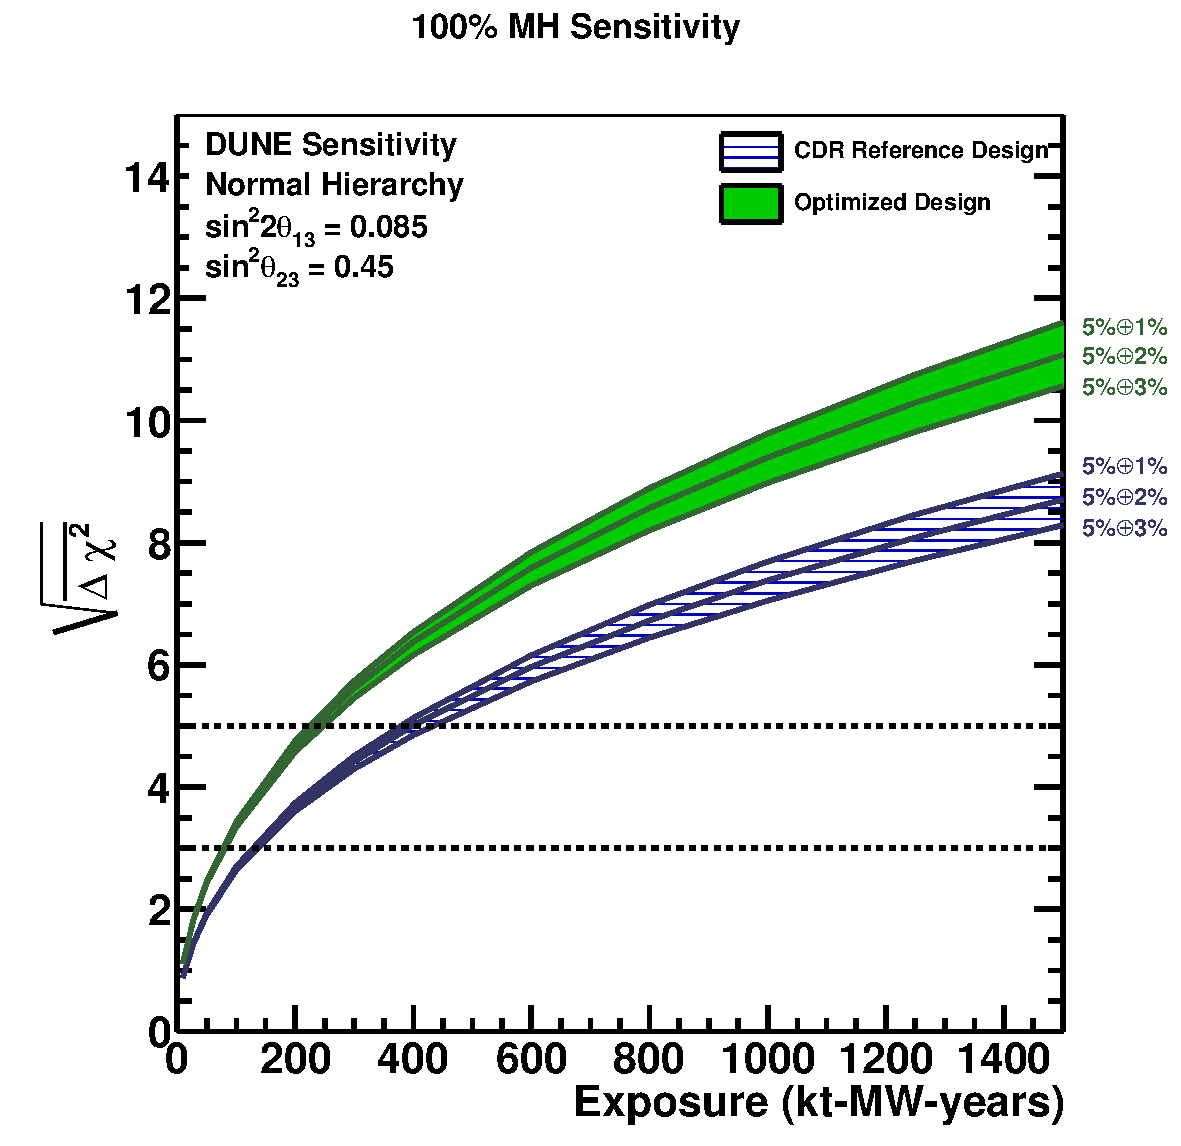
\includegraphics[width=0.32\linewidth]{volume-physics/figures/mh_exp_syst.pdf}
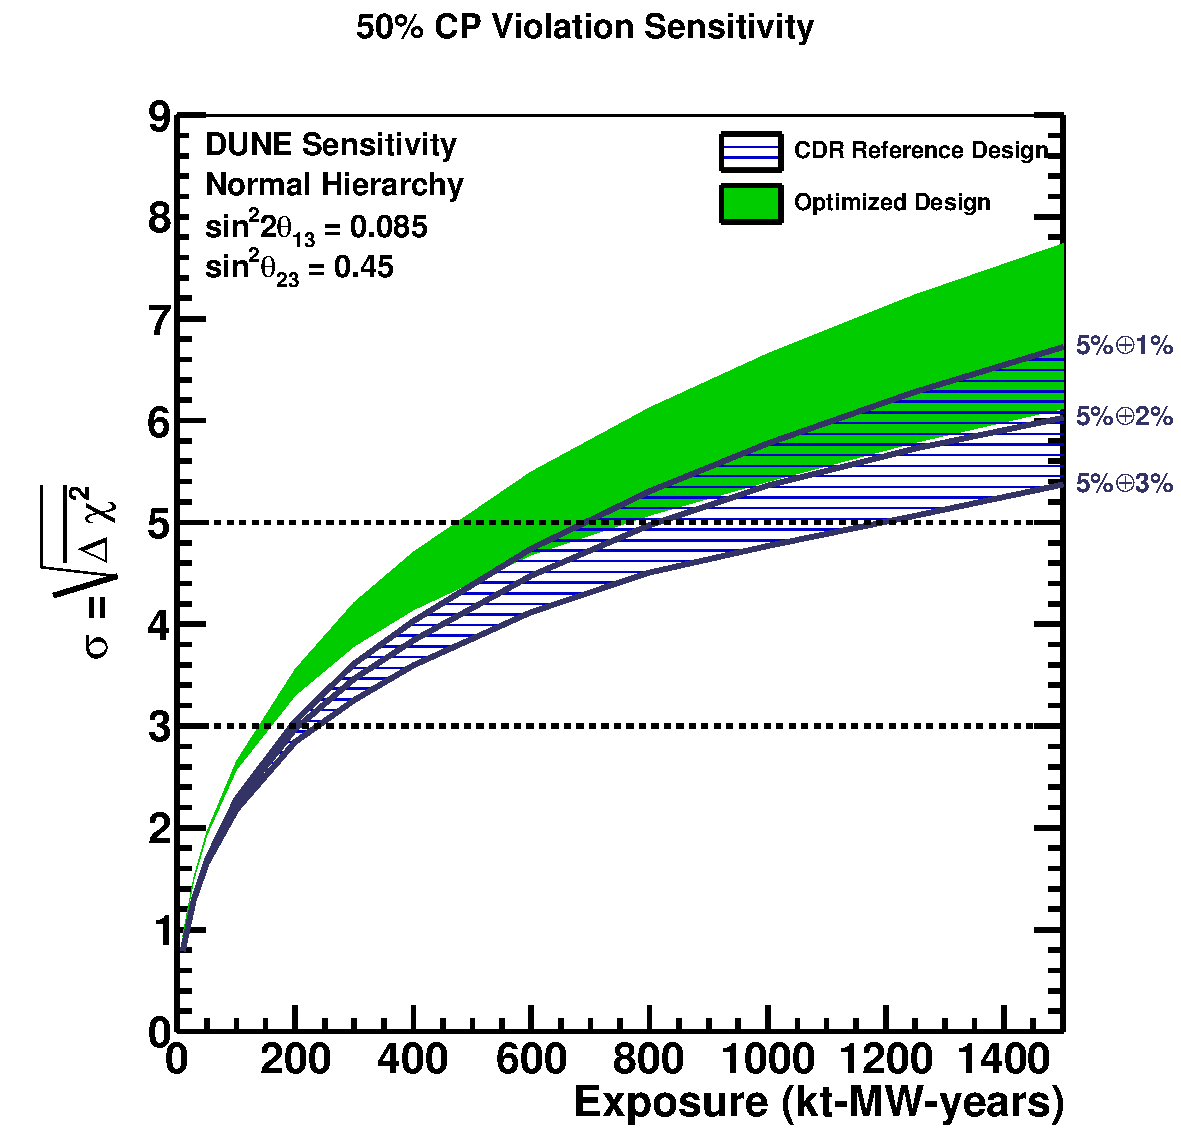
\includegraphics[width=0.32\linewidth]{volume-physics/figures/cpv50_exp_syst.pdf}
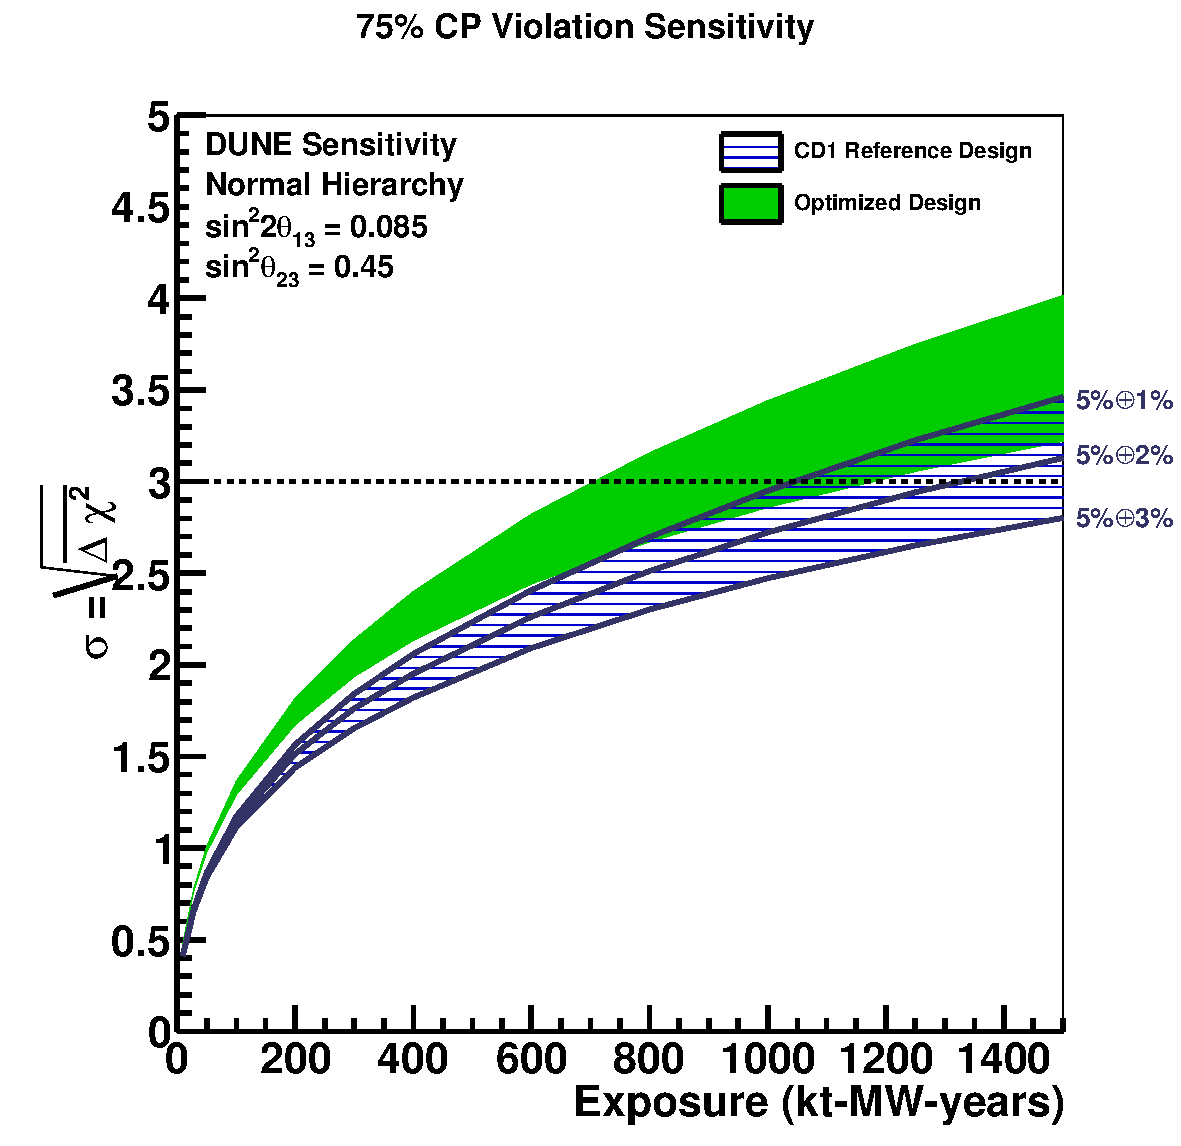
\includegraphics[width=0.32\linewidth]{volume-physics/figures/cpv75_exp_syst.pdf}
\caption{Expected sensitivity of DUNE to determination of the neutrino mass
  hierarchy (left) and discovery of CP violation, i.e. $\delta_{CP} \ne$ 0 or $\pi$,
  (middle, right) as a function of exposure in kt-MW-years, assuming 
  equal running in neutrino and antineutrino mode, for a range of values for
  the \nue and \anue signal normalization uncertainties from $5\%\oplus3\%$ to
  $5\%\oplus1\%$. The sensitivities quoted
  are the minimum sensitivity for 100\% of \deltacp values in the case of 
  mass hierarchy and 50\% of \deltacp values (middle) or 75\% of \deltacp values (right)
  in the case of CP violation. The two bands on each plot represent a range of potential
  beam designs: the blue hashed band is for the CDR Reference Design and the solid green
  band is for the Optimized Design. 
  Sensitivities are for true normal hierarchy; neutrino mass hierarchy
  and $\theta_{23}$ octant are assumed to be unknown.}
\label{fig:exp_systs}
\end{figure}
%
%% \begin{figure}[!htbp]
%% \centering
%% \includegraphics[width=0.32\linewidth]{volume-physics/figures/
%% \includegraphics[width=0.32\linewidth]{volume-physics/figures/
%% \includegraphics[width=0.32\linewidth]{volume-physics/figures/
%% \caption{Expected sensitivity of DUNE to determination of the neutrino mass
%%   hierarchy (left) and discovery of CP violation, i.e. $\delta_{CP} \ne$ 0 or $\pi$,
%%   (middle, right) as a function of exposure in kt-MW-years, assuming 
%%   equal running in neutrino and antineutrino mode, for a range of values for
%%   the \nue and \anue signal normalization uncertainties from $5\%\oplus3\%$ to
%%   $5\%\oplus1\%$. The sensitivities quoted
%%   are the minimum sensitivity for 100\% of \deltacp values in the case of 
%%   mass hierarchy and 50\% of \deltacp values (middle) or 75\% of \deltacp values (right)
%%   in the case of CP violation. The two bands on each plot represent a range of potential
%%   beam designs: the blue hashed band is for the CDR Reference Design and the solid green
%%   band is for the Optimized Design. 
%%   Sensitivities are for true normal hierarchy; neutrino mass hierarchy
%%   and $\theta_{23}$ octant are assumed to be unknown.}
%% \label{fig:escale_systs}
%% \end{figure}

The impact of systematic uncertainty on the CP violation sensitivity
is obvious in Fig.~\ref{fig:exp_systs}; the \nue signal normalization uncertainty must
be understood at the level of $5\% \oplus 2\%$ in order to reach 5$\sigma$ sensitivity for
75\% of \deltacp values with exposures less than $\sim$900~kt-MW-years in the case of the
Optimized Design. Specifically, the absolute normalization of the \numu sample must be known to
$\sim$5\% and the normalization of the \nue sample,
relative to the \anue, \numu, and \anumu samples after all constraints from
external, near detector, and far detector data have been applied, must be determined 
at the few percent level. This level of systematic uncertainty sets the capability and
design requirements for all components of the experiment, including the beam design, and the
near and far detectors.


%
\subsection{Ongoing Study of Systematic Uncertainties}
\label{sec:syst_studies_ind}
Detailed evaluation of systematic uncertainties for DUNE is ongoing. In many cases plans for studies
have been developed but have not yet been executed. In general, each systematic will be studied both by
propagating its uncertainty to oscillation analyses to evaluate the resultant degradation of the sensitivity
and by ensuring the varied model parameter and its allowed range gives proper coverage, i.e., truly encapsulates
the lack of knowledge of the process/effect in question. Estimates for systematics constraints for
propagation studies will be varied between current external knowledge to evaluate what would be possible in the
absence of a DUNE near detector and conservative and optimistic projections
for ND performance. In cases where systematic uncertainty is shown to degrade the oscillation parameter
measurement sensitivities, the required constraints will become detector performance requirements.
The details of these studies is beyond the scope of this document, however the conclusions from some
initial studies and an overview of each source of systematic uncertainty is laid out in the remainder of this section.

Initial studies using a Fast Monte Carlo with a parameterized detector response
predict 2-3\% statistical uncertainties on the absolute flux using fully 
leptonic neutrino interactions for which high-precision cross-section predictions 
exist. Specifically,
the statistical uncertainty is expected to be 2\% for neutrino-electron
scattering ($E_\nu<5$~GeV) and 3\% for inverse muon decay ($E_\nu>11$~GeV).
Relative normalization using the low-$\nu_0$ method is
expected to constrain the flux shape and the near/far flux ratio to 1-2\%.
Studies using a multi-sample fit  to constrain the flux with simulated near detector
event samples show significant constraints on all flux
uncertainties. The post-fit uncertainty 
in most flux bins for a preliminary fit is less
than 5\%, which is the uncorrelated \numu signal normalization
uncertainty assumed by the sensitivity calculations. 

Results from a fit to Fast MC simulation of all four far detector samples
(\nue, \anue, \numu, \anumu) significantly
constrains cross-section systematic uncertainty even in the case where many
cross-section parameters are allowed to vary simultaneously within their
GENIE uncertainties. As seen in the example shown in Figure
\ref{fig:MAresqesyst}, 
a fit in which both $M_A^{QE,CC}$ and 
$M_A^{RES,CC}$ are allowed to vary within their GENIE uncertainties 
($\pm$20\%), which could significantly alter the energy distribution of the 
the selected events, results in a dramatic reduction in sensitivity if one 
considers only the $\nu_e$ appearance signal without constraint from the 
$\bar{\nu}_e$ and $\nu_{\mu}$/$\bar{\nu}_{\mu}$ samples.
In contrast, for a four sample fit,
this same parameter variation results in only a small reduction in
sensitivity to CP violation.
This result includes a 10\% uncertainty in the $\nu/\bar{\nu}$
cross-section ratio and a 2.5\% uncertainty in the $\nu_e/\nu_{\mu}$
cross-section ratio.
Preliminary studies also
demonstrate significant constraint on cross-section systematics from the 
near detector. The validity of the GENIE model parameter uncertainties are being studied 
via comparisons with available data (e.g. MINERvA), and alternate models (e.g. the 
Intranuke intranuclear rescattering model and related uncertainties will be compared with GiBUU).
These comparisons are a high priority of the whole neutrino community as well as the DUNE collaboration.
\begin{figure}[!htbp]
\centering
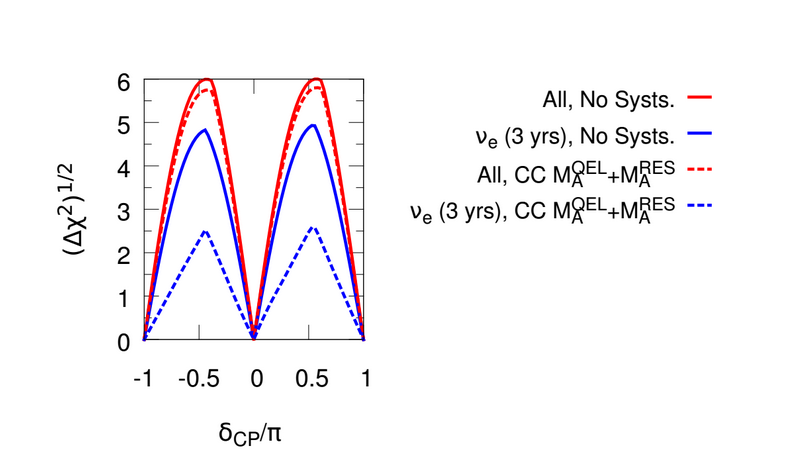
\includegraphics[width=0.8\linewidth]{volume-physics/figures/CPV_MARESQE.png}
\caption{An example CP violation sensitivity calculated using inputs from the 
  FastMC in a fit to all four ($\nu_e$, $\overline\nu_e$, $\nu_{\mu}$, 
  $\overline\nu_{\mu}$) samples (red) and a fit to the $\nu_e$ appearance sample 
  only (blue), for the case of no systematic uncertainty (solid) and the case in
  which both $M_A^{QE,CC}$ and $M_A^{RES,CC}$ are allowed to vary with a
  1$\sigma$ uncertainty of 20\% (dashed). This example was taken from an earlier
  DUNE study, so the absolute sensitivity can not be compared with the DUNE 
  sensitivities presented in this document.}
\label{fig:MAresqesyst}
\end{figure}

Uncertainty stemming from simulations of the interactions between hadrons
exiting the primary interaction vertex and the nuclear medium, and detector effects
such as resolutions and energy scale uncertainty, are somewhat more difficult to address with early
simulation efforts. However, in analogy to the treatment of cross-section uncertainty described above,
the effect of varying nuclear interaction parameters within their GENIE
uncertainties and comparisons of GENIE predictions to those of other
event generators are in progress.
Efforts to improve modeling of nuclear interactions and to develop 
reconstruction and analysis tools for a full Monte Carlo simulation are also underway. 
At the same time,
a number of test-beam and prototype experiments, including the DUNE 35-t prototype,
LARIAT, CAPTAIN, and the CERN neutrino platform experiments, are being designed and built to reduce these
uncertainties with experimental data.

The two main sources of uncertainty in the beam simulation come from variations in the beam optics
($\mathcal{O}$(1\%)) and uncertainties in the hadron production models ($\mathcal{O}$(10\%)).
Beam optics have been studied in detail, and while the variations in the flux produced by these uncertainties
lead to large uncertainties in the FD-only fits, they are easily constrained by the ND. Software tools that
allow reweighting of neutrinos based on their parent hadrons have been developed by MINERvA; we are working with
them port those tools to DUNE. In the meantime MINERva has agreed to provide their flux covariance matrix
that details the flux rate and shape uncertainties prior to ND constraints. We will combine this with DUNE
simulations to project reasonable hadron production uncertainties to ND and FD analyses.

OUTLINE ONLY AT THIS POINT, TO BE FILLED IN FURTHER
Each cross section model has uncertainties. In most cases these come from the hadron tensor part of the
calculation. These sources of uncertainty will be discussed in the context of nuclear models later in this
section. Primary interaction uncertainties are specific to each model.

  Coherent scattering:

  Quasi-elastic processes: these interactions are defined by low 4-momentum transfer and no excitation,
    or breakup of the struck nucleon

  Resonance production:

  Deep inelastic scattering:

The model of the initial nuclear state and final-state interactions have large effects on the
expected observables ...
